\documentclass[conference]{IEEEtran}
\IEEEoverridecommandlockouts
\usepackage{cite}
\usepackage{amsmath,amssymb,amsfonts}
\usepackage{graphicx}
\usepackage{booktabs}
\usepackage{textcomp}
\usepackage{xcolor}
\usepackage{url}
\usepackage{balance}
\graphicspath{{figures/}}

% ---------------------------------------------------------------------------
% Every number in this manuscript comes from research/results/results.json,
% produced by research/run_research.py. Tables are \input from tables/*.tex,
% which research/make_outputs.py generates from the same file.
% ---------------------------------------------------------------------------

\begin{document}

\title{Do Baseline-Relative Heart-Rate Features Help Recognize Induced Stress in Unseen Participants? A Confound-Aware Evaluation on the QoL\_Stress Consumer-Wearable Dataset}

\author{\IEEEauthorblockN{Author Name}
\IEEEauthorblockA{\textit{Department of Engineering}\\
\textit{College / University Name}\\
City, Country\\
email@example.com}}

\maketitle

\begin{abstract}
Wearable stress models often generalize poorly to unseen people. Expressing physiological features relative to each person's own baseline is a common remedy, but its benefit under strictly participant-independent testing, and its interaction with protocol confounds, has received limited direct attention in the reviewed literature. We study this on QoL\_Stress, a public PhysioNet dataset of 66 adults wearing a consumer Fitbit Charge~6 during a relaxation phase followed by a Stroop/video-game stress phase. Phases were reconstructed from questionnaire timestamps, and 57 participants met the quality criteria. We compared absolute heart-rate features (A) with features relative to a label-free 3-min resting calibration (R) that was excluded from scoring. The evaluation used participant-wise 5-fold cross-validation with identical folds, cluster-bootstrap intervals and Holm-corrected Wilcoxon tests. For 60-s windows, R or A+R raised balanced accuracy (BA) by 0.024--0.041 for logistic regression, random forest and support vector machine (best 0.613 vs.\ 0.573). The gain held for all 10 repeated fold assignments, but no paired test remained significant after correction. Confound controls were decisive: time since recording start alone reached a BA of 0.953, and heart-rate features separated early from late relaxation windows with a BA of 0.553--0.570. In temporally matched windows, the relative-feature advantage disappeared for logistic regression. Phase-level EDA and ECG-derived heart-rate variability did not significantly improve classification, and no model beat a mean predictor for STAI-S or PSS-14 scores. Baseline-relative features thus give small, consistent but statistically fragile gains, and on this dataset much of the detectable signal is confounded with time-on-task.
\end{abstract}

\begin{IEEEkeywords}
wearable sensing, stress detection, heart rate, personalization, participant-independent evaluation, data leakage, consumer wearables
\end{IEEEkeywords}

% ===========================================================================
\section{Introduction}
Psychological stress produces measurable autonomic responses. These include changes in heart rate (HR), heart-rate variability (HRV) and electrodermal activity (EDA), so wrist-worn sensors are attractive for continuous, unobtrusive monitoring~\cite{giannakakis2022review,schmidt2019review,kim2018hrv}. Laboratory studies with research-grade sensors report high accuracy for binary stress detection~\cite{schmidt2018wesad}. A systematic review, however, found that most wearable stress models are trained and tested on small single datasets and generalize poorly~\cite{vos2023generalizable}. Models also transfer badly across study protocols~\cite{mishra2020reproducibility}. Two difficulties recur:
\begin{itemize}
\item \textbf{Inter-individual variability.} Resting HR differs more between people than a stressor changes it within one person.
\item \textbf{Optimistic evaluation.} Windows from the same person in both training and test data inflate accuracy~\cite{saeb2017usecase}, and small-sample cross-validation (CV) has wide error bars~\cite{varoquaux2018cv}.
\end{itemize}

Personalization addresses the first difficulty. Some systems normalize each person's features with that person's own data~\cite{hovsepian2015cstress}. Others calibrate generic models with labelled samples from the target person~\cite{nkurikiyeyezu2020person,sah2021personalization}, or train fully personal models~\cite{tervonen2020som}. These approaches answer different questions from the one asked here. Labelled calibration presumes that the target user can label their own stress episodes. Within-person evaluation does not test generalization to new people. Normalization that uses all of a person's data, as in~\cite{hovsepian2015cstress}, implicitly sees both the stressed and the relaxed states. In the literature we reviewed, we found limited evidence that isolates the effect of \emph{label-free} baseline-relative features on \emph{unseen} participants with the same test participants and folds for both arms, particularly for consumer-grade HR. We also found limited evidence that checks whether such gains survive controls for the fixed order of laboratory protocols.

This paper studies that question on QoL\_Stress~\cite{calvo2026qolstress}, a recently released PhysioNet dataset~\cite{pollard2026physionet} recorded with a consumer Fitbit Charge~6. No modelling results on this dataset had been published at the time of writing; the dataset authors' own manuscript is in preparation~\cite{calvo2026qolstress}. We ask:
\begin{itemize}
\item \textbf{RQ1:} Under participant-independent evaluation, do HR features relative to a label-free resting calibration classify relax and induced-stress windows better than absolute HR features?
\item \textbf{RQ2:} Do phase-level EDA and ECG-derived HRV add information beyond HR?
\item \textbf{RQ3:} How strongly do the splitting strategy and the fixed relax-then-stress order (time-on-task) affect the conclusions?
\end{itemize}

\textbf{Contributions.} The contributions are evaluative; no new algorithm is proposed.
\begin{itemize}
\item A documented, reproducible protocol that reconstructs the experimental phases of QoL\_Stress from questionnaire timestamps and defines a label-free calibration period that is excluded from scoring.
\item A paired ablation of absolute, relative-only and combined HR features across three classifiers. It uses identical participant-wise folds, cluster-bootstrap confidence intervals, Holm-corrected tests, repeated CV and nested hyper-parameter tuning.
\item Confound and leakage controls rarely reported in the reviewed studies: record-wise vs.\ participant-wise CV, a time-only classifier, temporally matched windows and a same-condition drift classifier. These show that most of the detectable signal cannot be separated from time-on-task.
\item A validated R-peak pipeline for the 30-s, 250~Hz Fitbit ECG, and a segment-level evaluation of EDA and HRV with an explanation of why these signals carry little phase information under this protocol.
\end{itemize}

% ===========================================================================
\section{Related Work}
\subsection{Wearable physiological stress detection}
Early work showed that skin conductance and HR track driver stress~\cite{healey2005driving}. Reviews summarize HR, HRV and EDA as the most consistently stress-sensitive wearable signals~\cite{giannakakis2022review,schmidt2019review}, with stress typically reducing parasympathetic HRV indices~\cite{kim2018hrv}. WESAD~\cite{schmidt2018wesad} became a standard benchmark. It has 15 participants with chest and wrist research sensors and reports up to 93\% accuracy for stress vs.\ non-stress.

Laboratory models degrade in daily life. Context and activity recognition were needed for usable field detection~\cite{gjoreski2017context}, and reviews describe a persistent gap between laboratory and field performance~\cite{can2019survey}. Smartwatch sensors without EDA can support user-independent detection given sufficiently long windows~\cite{siirtola2019smartwatch}. Consumer Fitbit HR rises by a few beats per minute during self-reported stressors in students~\cite{pakhomov2020fitbit}, but that study analysed responses within each subject rather than evaluating a classifier on new people. Optical HR accuracy varies across devices and worsens during activity~\cite{bent2020optical}, which is relevant for consumer devices. Field datasets such as nurses' Empatica recordings~\cite{hosseini2022nurses} complement laboratory datasets.

\subsection{Personalization}
Individual differences motivate personalization. Large daily-life cohorts show heterogeneous "digital phenotypes" of stress response~\cite{smets2018digital}. Multitask models with person-specific components improve next-day mood and stress forecasts~\cite{taylor2020multitask}. Personal self-organizing maps reach high laboratory accuracy, but about 60\% in the field regardless of the degree of personalization~\cite{tervonen2020som}.

Calibrating a generic model with labelled samples from the target person improved accuracy substantially in~\cite{nkurikiyeyezu2020person}. Retraining a leave-one-subject-out (LOSO) model on held-out-subject data helped in a WESAD preprint~\cite{sah2021personalization}. Both approaches require labelled data from the target person. cStress normalizes each participant's features with that participant's own data and validates on new cohorts~\cite{hovsepian2015cstress}. In the reviewed sources, however, the contribution of normalization was not isolated by an ablation on the same test participants.

\subsection{Evaluation pitfalls}
Record-wise CV can greatly overestimate accuracy compared with subject-wise CV when the use case involves new individuals~\cite{saeb2017usecase}. CV error bars at sample sizes typical of physiological studies are wide~\cite{varoquaux2018cv}. Cross-study testing exposes poor reproducibility~\cite{mishra2020reproducibility}, and a systematic review highlights small datasets, labelling protocols and statistical power as recurring weaknesses~\cite{vos2023generalizable}.

\subsection{Positioning}
Unlike~\cite{nkurikiyeyezu2020person,sah2021personalization}, our calibration uses no labels from the test person. Unlike~\cite{tervonen2020som}, every test participant is unseen. Unlike~\cite{hovsepian2015cstress}, the baseline comes only from a pre-evaluation rest period, and the effect of normalization is isolated by a paired ablation. A transductive per-person $z$-score, which uses all of a person's windows, is reported only as an optimistic reference. Finally, we pair the comparison with explicit time-on-task controls, which we did not find reported for the reviewed laboratory datasets. A targeted, non-systematic search may have missed related studies; Section~\ref{sec:limits} discusses this.

% ===========================================================================
\section{Dataset and Problem Formulation}
\subsection{Source and protocol}
QoL\_Stress v1.0.0~\cite{calvo2026qolstress} (CC~BY~4.0) contains data from 66 healthy adults (39 male, 27 female; age 29.7$\pm$6.9 years, range 22--53). According to the \texttt{job\_category} field, participants were researchers and staff at a research institute; \emph{they were not students}.

Each session lasted about 30~min:
\begin{enumerate}
\item The participant completed the PSS-14~\cite{cohen1983pss} and watched a guided relaxation video.
\item A 30-s ECG and an EDA recording of up to 2~min were taken, followed by the STAI-S~\cite{spielberger1983stai}.
\item The participant performed a Stroop colour test~\cite{stroop1935} and played the video game Geometry Dash.
\item A second ECG and EDA recording and a second STAI-S followed.
\end{enumerate}
HR was recorded throughout with a Fitbit Charge~6. Calendar dates were removed; clock times were retained. Table~\ref{tab:dataset} lists the inspected files.

\begin{table}[t]
\caption{QoL\_Stress files as inspected (rows and unique participant IDs).}
\label{tab:dataset}
\centering\footnotesize
\resizebox{\columnwidth}{!}{\begin{tabular}{@{}llrr@{}}
\toprule
File & Content & Rows & IDs \\
\midrule
\texttt{participants.csv} & Demographics & 66 & 66 \\
\texttt{fitbit\_heart\_rate\_per\_second.csv} & Fitbit HR, irregular ($\approx$2 s) & 54,462 & 66 \\
\texttt{fitbit\_heart\_rate\_per\_minute.csv} & Fitbit HR per minute & 2,131 & 66 \\
\texttt{fitbit\_heart\_rate\_summary.csv} & Daily HR-zone minutes & 264 & 66 \\
\texttt{stai.csv} & STAI-S after each phase & 132 & 66 \\
\texttt{pss\_14.csv} & PSS-14 (past month) & 66 & 66 \\
\texttt{eda.csv} & EDA per phase & 20,094 & 64 \\
\texttt{ecg.csv} & 30-s ECG per phase (250 Hz) & 132 & 66 \\
\bottomrule
\end{tabular}
}
\end{table}

\subsection{Phase reconstruction and eligibility}
The Fitbit HR files contain only a participant ID, a clock time and a value in bpm, with no phase label. Each STAI-S answer, however, has a phase label and a clock time. In 65 of 66 sessions, the stress STAI-S follows the relax STAI-S, and HR recording ends close to the second STAI-S. We therefore treat each STAI-S timestamp as the end of its phase. This is an assumption; the dataset documentation does not state it.

ECG reading times were not used for alignment. For 13 eligible participants they fall outside the reconstructed phase, mostly offset by about 54~min, which suggests a clock offset.

Let $t_0$ be the first HR sample and let $\tau_r$ and $\tau_s$ be the relax and stress STAI-S times. The periods are defined as:
\begin{itemize}
\item calibration: $[t_0, t_0{+}3~\mathrm{min})$;
\item relax evaluation: $[t_0{+}3, \tau_r{-}2)$~min;
\item stress evaluation: $[\tau_r{+}1, \tau_s{-}2)$~min.
\end{itemize}
The guard bands remove questionnaire completion and the phase transition (Fig.~\ref{fig:timeline}).

A participant is eligible if all of the following hold:
\begin{itemize}
\item both timestamps are valid and in the expected order;
\item the calibration period has at least 45 samples;
\item each evaluation period is at least 3~min long and contains at least two valid 60-s windows;
\item HR recording does not end before the stress period.
\end{itemize}
57 participants were eligible. The exclusions were six for sparse calibration, one for late HR start, one for early HR end and one for a sparse segment.

HR samples outside 30--220~bpm and duplicate (ID, time) samples are removed; none occurred. No interpolation or forward filling is applied.

\begin{figure}[t]
\centering
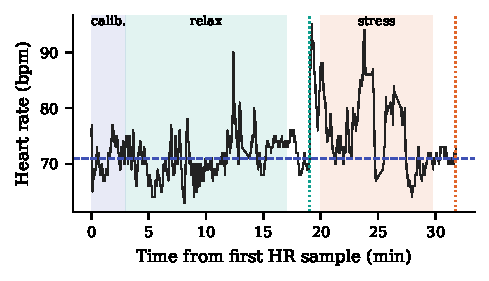
\includegraphics[width=\columnwidth]{fig2_timeline}
\caption{Fitbit HR of one eligible participant (real data). Shaded areas: calibration (blue), relax evaluation (teal) and stress evaluation (orange) periods after guard bands. Dotted lines: STAI-S timestamps. Dashed line: calibration median.}
\label{fig:timeline}
\end{figure}

\subsection{Prediction target}
The \textbf{primary target} is the protocol phase (relax $=0$, induced stress $=1$) of non-overlapping 60-s windows. This is the only label defined at the moment level. It describes an experimental condition, not perceived stress.

The data contain 746 relax and 471 stress windows. Each participant contributes a median of 20 windows (range 13--40), and each window contains a median of 28 HR samples. The evaluation periods last a median of 14.4~min for relax and 9.0~min for stress.

PSS-14 refers to the previous month, and STAI-S is reported only twice per person. Both are analysed only as secondary regression targets and never as window labels.

As a manipulation check, STAI-S rose from $33.6\pm7.3$ after relaxation to $36.9\pm8.8$ after stress (Wilcoxon $p<10^{-4}$; 37 higher, 11 equal, 9 lower). Mean window HR was higher in the stress phase for 43 of the 57 participants.

% ===========================================================================
\section{Methodology}
Fig.~\ref{fig:workflow} summarizes the implemented pipeline.

\begin{figure*}[t]
\centering
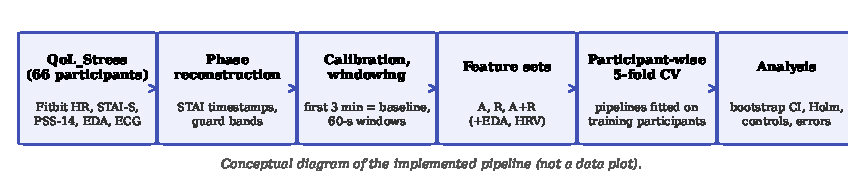
\includegraphics[width=0.95\textwidth]{fig1_workflow}
\caption{Implemented analysis pipeline (conceptual diagram, not a data plot). All fitted preprocessing is learned from the training participants of each fold.}
\label{fig:workflow}
\end{figure*}

\subsection{Features}
Let $h=\{h_1,\dots,h_n\}$ be the valid HR samples in a window, recorded at times $t_i$. Let $\mu_c$, $m_c$ and $\sigma_c$ be the mean, median and standard deviation of the participant's calibration samples, and let $\tilde\sigma=\max(\sigma_c, 1~\mathrm{bpm})$.

\textbf{Absolute features (A)} are the mean $\bar h$, the median $\tilde h$, the standard deviation $s_h$, the minimum, the maximum, the interquartile range, and the least-squares slope $\beta$ of $h$ against $t$ in bpm/min.

\textbf{Baseline-relative features (R)} are
\begin{equation}
\bar h - m_c,\quad \tilde h - m_c,\quad \frac{\bar h}{m_c},\quad \frac{\bar h-\mu_c}{\tilde\sigma},\quad \frac{s_h}{\tilde\sigma}.
\end{equation}
R uses no labels. It also uses no data from the evaluation periods, so it could be computed at deployment after a short rest.

The set \textbf{A+R} combines both. Two further sets serve as references or controls:
\begin{itemize}
\item \textbf{Zt} $z$-scores every A feature with the mean and standard deviation of \emph{all} of that participant's evaluation windows. This is cStress-like normalization~\cite{hovsepian2015cstress}. It is not deployable and is reported only as an optimistic reference.
\item \textbf{T} is the time since $t_0$ alone, used as a control.
\end{itemize}

At segment level (the last 5~min of each phase's evaluation period; 114 segments), we add two further feature groups:
\begin{itemize}
\item \textbf{EDA:} the mean and standard deviation of the skin-conductance level, and the fraction of samples with activation, using rows with \texttt{valid\_data} set and $\texttt{time\_sec}\geq0$.
\item \textbf{ECG HRV:} the derived HR, SDNN and RMSSD~\cite{taskforce1996hrv} from the 30-s ECG at 250~Hz.
\end{itemize}

R-peaks are detected with a simplified Pan--Tompkins pipeline~\cite{pan1985qrs}: a 5--15~Hz band-pass filter, differentiation, squaring, 150-ms moving integration, and peak picking with a 300-ms refractory period. Each peak is then refined to the maximum of the band-passed signal within $\pm$60~ms. RR intervals outside 300--2000~ms, or more than 30\% from the median, are rejected, and a recording needs at least 15 RR intervals.

Of the 132 recordings, 123 were usable. Eighteen contained a single non-numeric sample, which was bridged by interpolation over a 4-ms gap. Against the HR reported by the device for normal-sinus-rhythm recordings ($n=114$), the derived HR had a mean absolute error of 1.07~bpm, a bias of $+0.67$~bpm and 95\% limits of agreement of $[-1.66, 3.00]$~bpm. The largest error was 4.3~bpm.

\subsection{Models and leakage prevention}
We compare four models, using scikit-learn~\cite{pedregosa2011sklearn}:
\begin{itemize}
\item a majority-class baseline;
\item logistic regression (LR);
\item a random forest (RF) with 300 trees and \texttt{min\_samples\_leaf}$=5$;
\item an RBF support vector machine (SVM) with $C=1$ and $\gamma=\textit{scale}$.
\end{itemize}
The three real models use balanced class weights. Every model is a pipeline of median imputation, standardization and the classifier, so all fitted preprocessing sees only the training participants.

Hyper-parameters are fixed in advance. Nested tuning, with an inner grouped 4-fold CV on the training participants, is run only as a sensitivity analysis.

\subsection{Evaluation protocol}
Participants are shuffled with seed 42 and assigned to five folds. \emph{The same assignment is used for every feature set and model}, which makes all comparisons paired. The code asserts that no participant appears in both the training and test sets of any fold. Each fold trains on 45--46 participants and tests on 11--12.

Metrics are computed from pooled out-of-fold predictions: balanced accuracy (BA), macro-F1, per-class recall, ROC-AUC (from probabilities or decision values) and the confusion matrix. BA is also computed for each participant.

Uncertainty and significance are assessed in three ways:
\begin{itemize}
\item 95\% confidence intervals from a participant-cluster bootstrap with 2000 resamples; paired differences use the same resamples for both arms.
\item Two-sided Wilcoxon signed-rank tests~\cite{wilcoxon1945} on per-participant BA, with Holm correction~\cite{holm1979}. The window-level family has six tests (three models, each comparing R and A+R against A). The segment-level family has twelve tests.
\item Repeating the full CV with 10 alternative fold seeds, which shows sensitivity to the fold assignment.
\end{itemize}

\subsection{Confound and leakage controls}
\begin{enumerate}
\item \emph{Record-wise CV:} stratified 5-fold CV over windows that ignores participant identity, compared with participant-wise CV.
\item \emph{Time-only classifier:} T as the sole feature. This measures how separable the phases are from protocol order alone.
\item \emph{Temporally matched windows:} for each participant, the last three relax windows and the first three stress windows only. This minimizes the time separation between classes; the median gap is 4.6~min.
\item \emph{Same-condition drift control:} classifying the first vs.\ the second half of each participant's \emph{relax} windows. Any skill above chance here must come from drift, because the condition does not change.
\end{enumerate}

% ===========================================================================
\section{Experimental Setup}
All experiments were run with Python 3.12.0, NumPy 2.5.4, pandas 3.1.0, scikit-learn 1.8.0 and SciPy 1.18.1 on Windows 11 with an Intel 64-bit processor. The complete run took 381~s on a CPU.

The dataset fingerprint (a hash of the input files) is \texttt{6a342b432fcef3be}. The global seed is 42, and the repeated CV uses seeds 1000--1009.

The scripts, configuration and per-participant outputs are part of the project repository. The preprocessing code is shared with the accompanying research application.

% ===========================================================================
\section{Results}
\subsection{RQ1: absolute vs.\ baseline-relative HR features}
Table~\ref{tab:window} and Fig.~\ref{fig:window} report window-level performance. All real models exceeded the majority baseline (BA 0.500), but only modestly.

With absolute features, LR reached BA 0.578 [0.538, 0.616]. Replacing them with relative features raised BA for every model: LR 0.603, RF 0.574 and SVM 0.613 for R only, against 0.578, 0.535 and 0.573 for A. A+R performed similarly to R (0.602, 0.566 and 0.610).

The Zt reference, which uses future windows from both classes, gave the highest BA (LR 0.628), as expected for an optimistic procedure. Recall was asymmetric: with A+R and SVM, relax recall was 0.776 and stress recall 0.444.

\begin{table*}[t]
\caption{Window-level results under participant-wise 5-fold CV (57 participants, 1217 windows). BA with 95\% participant-cluster bootstrap CI. Zt is a non-deployable transductive reference. Time-only is a confound control.}
\label{tab:window}
\centering\footnotesize
\begin{tabular}{@{}llccccc@{}}
\toprule
Features & Model & BA [95\% CI] & Macro-F1 & Rec.$_\mathrm{relax}$ & Rec.$_\mathrm{stress}$ & AUC \\
\midrule
Absolute (A) & Majority & 0.500 [0.500, 0.500] & 0.380 & 1.000 & 0.000 & -- \\
Absolute (A) & LR & 0.578 [0.538, 0.616] & 0.578 & 0.662 & 0.495 & 0.604 \\
Absolute (A) & RF & 0.535 [0.502, 0.571] & 0.536 & 0.668 & 0.403 & 0.558 \\
Absolute (A) & SVM & 0.573 [0.538, 0.607] & 0.573 & 0.733 & 0.412 & 0.588 \\
\midrule
Relative only (R) & Majority & 0.500 [0.500, 0.500] & 0.380 & 1.000 & 0.000 & -- \\
Relative only (R) & LR & 0.603 [0.563, 0.642] & 0.603 & 0.700 & 0.505 & 0.605 \\
Relative only (R) & RF & 0.574 [0.538, 0.612] & 0.575 & 0.680 & 0.469 & 0.603 \\
Relative only (R) & SVM & 0.613 [0.572, 0.654] & 0.615 & 0.779 & 0.448 & 0.605 \\
\midrule
Absolute + relative (A+R) & Majority & 0.500 [0.500, 0.500] & 0.380 & 1.000 & 0.000 & -- \\
Absolute + relative (A+R) & LR & 0.602 [0.560, 0.642] & 0.602 & 0.682 & 0.522 & 0.608 \\
Absolute + relative (A+R) & RF & 0.566 [0.526, 0.605] & 0.566 & 0.680 & 0.452 & 0.579 \\
Absolute + relative (A+R) & SVM & 0.610 [0.566, 0.653] & 0.612 & 0.776 & 0.444 & 0.599 \\
\midrule
Transductive z-score & LR & 0.628 [0.579, 0.675] & 0.626 & 0.677 & 0.580 & 0.650 \\
Transductive z-score & RF & 0.611 [0.570, 0.651] & 0.611 & 0.701 & 0.520 & 0.635 \\
\midrule
Time only & LR & 0.953 [0.930, 0.975] & 0.949 & 0.948 & 0.958 & 0.986 \\
Time only & RF & 0.965 [0.943, 0.985] & 0.965 & 0.976 & 0.953 & 0.990 \\
\bottomrule
\end{tabular}

\end{table*}

\begin{figure}[t]
\centering
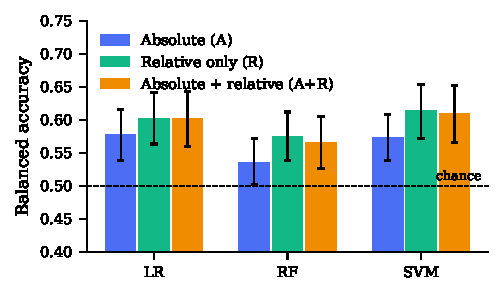
\includegraphics[width=\columnwidth]{fig3_window_ba}
\caption{Window-level balanced accuracy (95\% participant-cluster bootstrap CI) for absolute (A), relative-only (R) and combined (A+R) HR features.}
\label{fig:window}
\end{figure}

Table~\ref{tab:comp} reports the paired comparisons. All six pooled differences were positive, ranging from $+0.024$ to $+0.041$. The bootstrap probability that a difference was positive ranged from 0.89 to 0.99, and the 95\% CI excluded zero only for SVM ($+0.041$ [$+0.004$, $+0.077$] for R; $+0.037$ [$+0.008$, $+0.069$] for A+R).

Per-participant Wilcoxon tests gave $p=0.023$ and $p=0.026$ for SVM and $p\geq0.11$ for the other models. After Holm correction, every $p$ was at least 0.139.

Across 10 alternative fold assignments, R and A+R beat A in all 60 model-by-comparison-by-repeat cases. These repeats reuse the same participants, so they show robustness to the fold assignment, not independent replication. Per-participant improvements were mixed; for LR with A+R, 29 participants improved, 22 worsened and 6 were unchanged (Fig.~\ref{fig:pp}).

\begin{table*}[t]
\caption{Paired comparisons with the absolute feature set A (same participants and folds). $\Delta$BA pooled: difference in pooled BA with paired bootstrap 95\% CI. $\Delta$BA$_\mathrm{pp}$: mean per-participant difference. +/$-$/=: participants improved, worsened or tied. $p$: Wilcoxon signed-rank. $p_\mathrm{Holm}$: Holm-adjusted over six tests. Repeated CV: mean BA over 10 fold seeds (number of seeds in which the relative set won).}
\label{tab:comp}
\centering\footnotesize
\begin{tabular}{@{}llcccccc@{}}
\toprule
Model & Comparison & $\Delta$BA pooled [95\% CI] & $\Delta$BA$_\mathrm{pp}$ & +/$-$/= & $p$ & $p_\mathrm{Holm}$ & Repeated CV (wins) \\
\midrule
LR & R vs A & +0.024 [-0.012, +0.062] & +0.026 & 30/25/2 & 0.112 & 0.449 & 0.602 vs 0.579 (10/10) \\
LR & A+R vs A & +0.024 [-0.003, +0.054] & +0.022 & 29/22/6 & 0.114 & 0.449 & 0.595 vs 0.579 (10/10) \\
RF & R vs A & +0.039 [-0.002, +0.078] & +0.032 & 28/26/3 & 0.130 & 0.449 & 0.564 vs 0.547 (10/10) \\
RF & A+R vs A & +0.030 [-0.006, +0.063] & +0.022 & 27/26/4 & 0.214 & 0.449 & 0.575 vs 0.547 (10/10) \\
SVM & R vs A & +0.041 [+0.004, +0.077] & +0.042 & 38/18/1 & 0.023 & 0.139 & 0.604 vs 0.578 (10/10) \\
SVM & A+R vs A & +0.037 [+0.008, +0.069] & +0.037 & 32/19/6 & 0.026 & 0.139 & 0.600 vs 0.578 (10/10) \\
\bottomrule
\end{tabular}

\end{table*}

\begin{figure}[t]
\centering
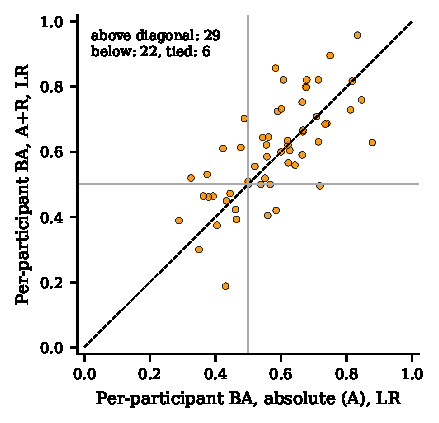
\includegraphics[width=0.8\columnwidth]{fig4_per_participant}
\caption{Per-participant BA for absolute (A) vs.\ combined (A+R) features with LR. Points above the diagonal are participants who benefited from the relative features.}
\label{fig:pp}
\end{figure}

The length of the calibration period mattered at 1~min, where BA was 0.569--0.584, but changed little between 2 and 3~min (0.591--0.613; Table~\ref{tab:cal}). Nested hyper-parameter tuning changed BA by at most $\pm$0.024, and A+R remained above A for every model (Table~\ref{tab:nested}).

\begin{table}[t]
\caption{Calibration-length sensitivity (window BA). The evaluation windows are identical in every row.}
\label{tab:cal}
\centering\footnotesize
\begin{tabular}{@{}lcccc@{}}
\toprule
& \multicolumn{2}{c}{R only} & \multicolumn{2}{c}{A+R} \\
Calibration & LR & SVM & LR & SVM \\
\midrule
1 min & 0.569 & 0.574 & 0.584 & 0.570 \\
2 min & 0.605 & 0.604 & 0.596 & 0.591 \\
3 min & 0.603 & 0.613 & 0.602 & 0.610 \\
\bottomrule
\end{tabular}

\end{table}

\begin{table}[t]
\caption{Fixed vs.\ nested-tuned hyper-parameters (window BA). Inner grouped 4-fold CV on the training participants only.}
\label{tab:nested}
\centering\footnotesize
\begin{tabular}{@{}llcc@{}}
\toprule
Features & Model & Fixed & Nested-tuned \\
\midrule
Absolute (A) & LR & 0.578 & 0.582 \\
Absolute (A) & RF & 0.535 & 0.551 \\
Absolute (A) & SVM & 0.573 & 0.571 \\
Absolute + relative (A+R) & LR & 0.602 & 0.613 \\
Absolute + relative (A+R) & RF & 0.566 & 0.590 \\
Absolute + relative (A+R) & SVM & 0.610 & 0.594 \\
\bottomrule
\end{tabular}

\end{table}

\subsection{RQ3: leakage and temporal confounds}
Fig.~\ref{fig:controls}(a) compares record-wise and participant-wise CV. Record-wise CV inflated BA by at most 0.018 for LR and SVM, by 0.027 for RF with A, and by 0.045 for RF with A+R. The inflation is therefore present but small here, and largest for the most flexible model.

The time-only control was the most important result. Time since recording start alone gave a BA of 0.953 with LR and 0.965 with RF, with an ROC-AUC of 0.986 and 0.990. Because the stress phase always followed the relax phase, any feature that drifts with time is confounded with the label.

The same-condition drift control confirms that such drift exists in HR. HR features classified the early vs.\ late half of the relax windows, which share the same condition, with BA 0.553--0.570. This is of the same order as the relax-vs-stress BA.

Within the stress phase, HR declined over time (median slope $-0.26$~bpm/min, Wilcoxon $p=0.019$). Within the relax phase, it did not change significantly (median $-0.08$~bpm/min, $p=0.78$).

\begin{figure*}[t]
\centering
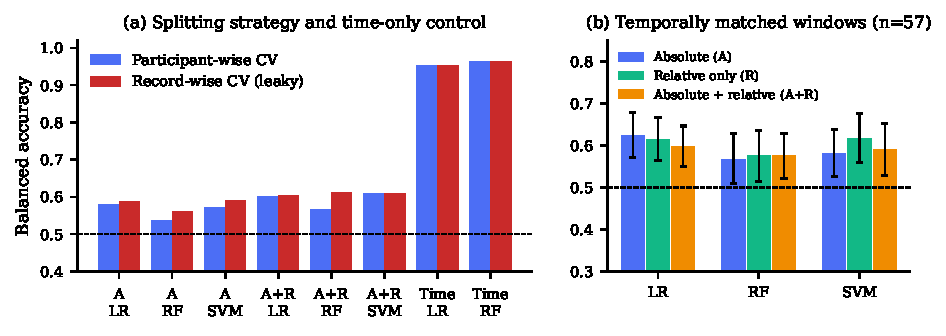
\includegraphics[width=0.95\textwidth]{fig6_controls}
\caption{(a) Participant-wise vs.\ record-wise (leaky) CV, and the time-only control. (b) Temporally matched windows (the last three relax and first three stress windows per participant; 342 windows) with 95\% bootstrap CI.}
\label{fig:controls}
\end{figure*}

In temporally matched windows (Fig.~\ref{fig:controls}(b)), absolute features with LR reached BA 0.623 [0.570, 0.678], which is \emph{higher} than R (0.614) and A+R (0.596). SVM still favoured R (0.617 vs.\ 0.582), but the confidence intervals overlapped widely. The relative-feature advantage seen in the full data is therefore not robust once the time separation between the classes is reduced.

\subsection{Error analysis}
With A+R and LR, the confusion matrix has 509 true relax, 237 false stress, 225 missed stress and 246 true stress windows (Fig.~\ref{fig:cm}).

Per-participant BA had a mean of 0.603 and an SD of 0.157. Fourteen of the 57 participants scored below 0.5, and 11 scored at least 0.75.

Per-participant BA correlated with the participant's own stress-minus-relax change in segment HR (Spearman $\rho=0.51$, $p<10^{-4}$). It did not correlate with the change in STAI-S ($\rho=0.10$, $p=0.48$), and its relation to baseline HR was weak ($\rho=-0.25$, $p=0.06$). The model therefore succeeds mainly for participants whose HR rose during the stress phase, whether or not they reported more anxiety.

Accuracy also depended on position (Fig.~\ref{fig:pos}). Stress windows were recognized best 2--4~min after the start of the stress period (accuracy 0.61--0.65) and worst near its end (0.33--0.47). The end of the stress period contained the post-task ECG and EDA recordings and the questionnaire lead-in.

In permutation importance on held-out folds, the strongest features for LR were the baseline ratio $\bar h/m_c$ (a BA drop of 0.097), $h_{\min}$ (0.083) and $s_h$ (0.042). Importances for RF were all below 0.01, consistent with redundancy among correlated features (Fig.~\ref{fig:imp}).

\begin{figure}[t]
\centering
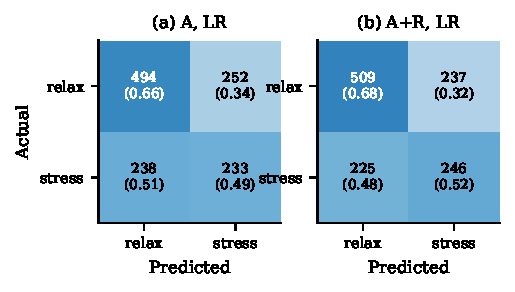
\includegraphics[width=\columnwidth]{fig5_confusion}
\caption{Pooled out-of-fold confusion matrices for LR with (a) absolute and (b) combined features. Row-normalized values are in parentheses.}
\label{fig:cm}
\end{figure}

\begin{figure}[t]
\centering
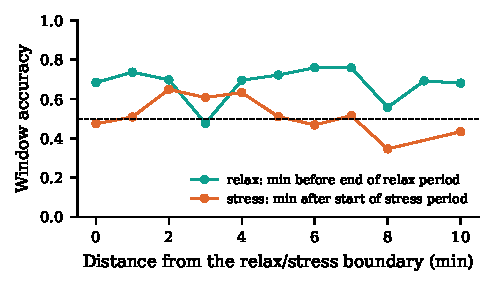
\includegraphics[width=\columnwidth]{fig8_position}
\caption{Window accuracy (A+R, LR) by distance from the relax/stress boundary. Bins with fewer than 20 windows are omitted; bin 10 pools all distances of 10~min or more.}
\label{fig:pos}
\end{figure}

\begin{figure}[t]
\centering
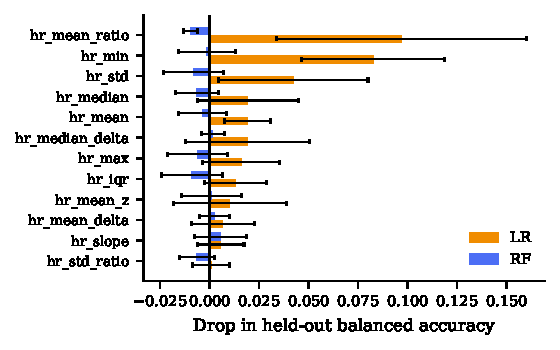
\includegraphics[width=\columnwidth]{fig7_importance}
\caption{Grouped permutation importance (drop in held-out BA, mean $\pm$ SD over folds, 20 repeats per fold) for the A+R feature set.}
\label{fig:imp}
\end{figure}

\subsection{RQ2: EDA and ECG-derived HRV at segment level}
Table~\ref{tab:seg} and Fig.~\ref{fig:seg} report the segment-level results. Absolute HR with LR gave BA 0.667 [0.579, 0.754]. The highest value, 0.702 [0.623, 0.781], came from RF with A+R+EDA+HRV. EDA and HRV alone gave 0.588--0.614.

None of the twelve comparisons with A was significant, either before (minimum $p=0.096$) or after Holm correction (every adjusted $p$ was 1.0). The largest mean per-participant gain, $+0.061$ for RF with A+R+EDA+HRV, had a paired bootstrap CI of $[-0.009, +0.140]$ for the pooled difference.

The HRV changes ran opposite to the usual stress response~\cite{kim2018hrv}. In the stress-phase recordings, RMSSD (median $+7.5$~ms, $p=0.019$) and SDNN ($+9.4$~ms, $p=0.025$) were \emph{higher} than in the relax-phase recordings, and the derived HR did not differ (median 67.4~bpm in both phases). This pattern is consistent with the ECG having been recorded after the stressor ended. Under this protocol, the phase-level ECG and EDA therefore probably capture recovery more than the stress response.

\begin{table}[t]
\caption{Segment-level BA [95\% CI] (57 participants, 114 segments). Imputed: missing feature values filled by median imputation inside each training fold.}
\label{tab:seg}
\centering\footnotesize
\resizebox{\columnwidth}{!}{\begin{tabular}{@{}lcccc@{}}
\toprule
Features & LR & RF & SVM & Imputed \\
\midrule
A & 0.667 [0.58, 0.75] & 0.640 [0.56, 0.72] & 0.640 [0.56, 0.72] & 0 \\
A+R & 0.675 [0.59, 0.75] & 0.640 [0.56, 0.72] & 0.640 [0.57, 0.71] & 0 \\
A+R+EDA & 0.667 [0.58, 0.75] & 0.693 [0.61, 0.77] & 0.623 [0.55, 0.69] & 18 \\
A+R+HRV & 0.667 [0.59, 0.75] & 0.684 [0.61, 0.76] & 0.632 [0.56, 0.71] & 27 \\
A+R+EDA+HRV & 0.632 [0.54, 0.71] & 0.702 [0.62, 0.78] & 0.623 [0.54, 0.70] & 45 \\
EDA+HRV only & 0.614 [0.54, 0.69] & 0.588 [0.51, 0.67] & 0.614 [0.54, 0.68] & 45 \\
\bottomrule
\end{tabular}
}
\end{table}

\begin{figure}[t]
\centering
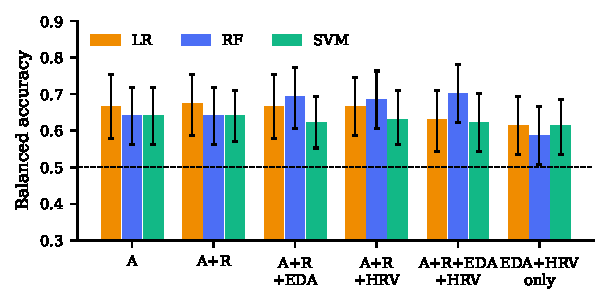
\includegraphics[width=\columnwidth]{fig9_segment}
\caption{Segment-level BA (95\% CI) when EDA and ECG-derived HRV are added to the HR features.}
\label{fig:seg}
\end{figure}

\subsection{Secondary targets}
Table~\ref{tab:reg} reports the regression results. For both STAI-S (per phase) and PSS-14 (per participant), no HR-based model achieved a lower mean absolute error (MAE) than predicting the training mean (MAE 6.67 and 6.51, respectively), and all $R^2$ values were at most 0.001.

\begin{table}[t]
\caption{Secondary regression targets: MAE / $R^2$ under participant-wise CV. Sets A, B (=A+R) and C (=A+R+EDA+device ECG HR) are as defined in the accompanying application.}
\label{tab:reg}
\centering\footnotesize
\resizebox{\columnwidth}{!}{\begin{tabular}{@{}llcccc@{}}
\toprule
Target & Set & Mean & Ridge & RF & SVR \\
\midrule
STAI-S & A & 6.67 / -0.04 & 7.25 / -0.21 & 7.24 / -0.20 & 7.07 / -0.21 \\
STAI-S & B & 6.67 / -0.04 & 7.30 / -0.26 & 7.41 / -0.22 & 7.19 / -0.22 \\
STAI-S & C & 6.67 / -0.04 & 7.37 / -0.28 & 7.38 / -0.25 & 6.99 / -0.19 \\
PSS-14 & A & 6.51 / -0.01 & 8.26 / -0.93 & 7.48 / -0.24 & 7.23 / -0.13 \\
PSS-14 & B & 6.51 / -0.01 & 9.23 / -1.38 & 7.02 / -0.13 & 6.97 / -0.09 \\
PSS-14 & C & 6.51 / -0.01 & 9.12 / -1.43 & 6.58 / 0.00 & 6.76 / -0.05 \\
\bottomrule
\end{tabular}
}
\end{table}

% ===========================================================================
\section{Discussion}
\textbf{Does personalization help?} The answer is a qualified yes, and only weakly. Relative features increased BA for every model and every fold assignment. That consistency matters, because the absolute-feature models were close to chance. However, the effect was small (about 0.02--0.04 BA), it did not survive multiple-comparison correction, and it did not hold in temporally matched windows. Within the limitations of this dataset, the evidence is insufficient to conclude that baseline-relative features improve recognition of induced stress in unseen participants. This is consistent with reports that personalization gains are modest when the target person contributes no labels~\cite{tervonen2020som}. It contrasts with the large gains reported when labelled target data are available~\cite{nkurikiyeyezu2020person}.

\textbf{What do the models learn?} The importance of the baseline ratio and the strong link between per-participant BA and each person's HR increase suggest the following. The models mostly detect an elevation of HR relative to rest, and they succeed for participants whose HR rose and fail for those whose did not. The lack of association with the change in STAI-S indicates that this elevation is not a reliable proxy for perceived anxiety. The time-only and drift controls show that part of what can be detected is simply \emph{when} a window occurred. Because the order of relaxation and stress was fixed, these effects cannot be disentangled with this dataset.

\textbf{Why are some models weaker?} RF benefited most from leaky record-wise splits and performed worst under participant-wise splits. This is consistent with flexible models memorizing person-specific HR levels, which is exactly what relative features remove~\cite{saeb2017usecase}. The record-wise inflation was nonetheless smaller here than often reported, plausibly because the class signal itself is weak.

\textbf{EDA and HRV.} The absence of a gain is explained by the protocol: the ECG and EDA were recorded after each phase's task. The higher HRV in the stress-phase recordings suggests post-task recovery. Recordings made \emph{during} the stressor would be needed to assess these modalities fairly.

\textbf{What the results do not establish.} We do not claim real-time stress detection, clinical validity, or transfer to other devices or populations. The results concern the classification of a laboratory condition in research-institute staff wearing a Fitbit.

% ===========================================================================
\section{Limitations and Threats to Validity}
\label{sec:limits}
\begin{itemize}
\item \textbf{Label validity.} Labels are protocol conditions, reconstructed from questionnaire timestamps under a stated assumption. They are not momentary self-reports, and the phase boundaries are approximate.
\item \textbf{Order confound.} Stress always followed relaxation. Time-on-task, fatigue, posture and the content of the questionnaires all co-vary with the label, as the time-only control shows. A counterbalanced protocol is required to separate them.
\item \textbf{Sample.} The analysis covers 57 eligible adults from one institution, with a male majority and a narrow age range; they were \emph{not students}. Small-sample CV has wide error bars~\cite{varoquaux2018cv}, and Table~\ref{tab:window} reports them.
\item \textbf{Sensing.} The study uses only optical HR from a consumer device, whose accuracy depends on motion~\cite{bent2020optical}. No activity data were available, so an activity-adjusted analysis was not possible. The HRV is ultra-short (30~s), shorter than standard recommendations~\cite{taskforce1996hrv}.
\item \textbf{Generalization.} There is no external or cross-dataset validation~\cite{mishra2020reproducibility}, and \emph{no validation on other consumer devices}, including the Amazfit watches that motivated this project.
\item \textbf{Analysis choices.} Window length, guard bands and calibration length were fixed in advance; only the calibration length was varied. The Wilcoxon tests on per-participant BA for segments are coarse, because each participant contributes only two segments.
\item \textbf{Literature search.} The search was targeted rather than systematic, so related ablations may exist in venues that were not searched.
\end{itemize}

% ===========================================================================
\section{Conclusion and Future Work}
We asked whether label-free, baseline-relative HR features help recognize an induced-stress condition in participants not seen during training, using a consumer-wearable dataset and a leakage-controlled, paired evaluation.

Relative features gave small and consistent improvements over absolute HR, but these were not statistically robust. The improvements disappeared when temporal separation was controlled. Phase-level EDA and HRV added no significant information under a protocol that records them after the stressor. HR features did not predict self-reported state or perceived stress.

The main contribution is evaluative. On QoL\_Stress, time-on-task explains a large share of what is learnable, and confound controls should accompany any reported accuracy.

Future work should:
\begin{itemize}
\item use counterbalanced or repeated relax/stress protocols;
\item capture physiology during the stressor;
\item collect momentary self-reports;
\item validate on other consumer devices, such as Amazfit, and on student populations;
\item compare label-free baselines with few-shot labelled calibration under the same participant-independent protocol.
\end{itemize}

\section*{Data and Code Availability}
QoL\_Stress is available from PhysioNet~\cite{calvo2026qolstress} under CC~BY~4.0. The analysis code, configuration and generated results accompany this manuscript.

\section*{Acknowledgment}
We thank the creators of the QoL\_Stress dataset and PhysioNet~\cite{pollard2026physionet} for making the data openly available.

\balance
\bibliographystyle{IEEEtran}
\bibliography{references}

\end{document}
